\section{Results}\label{sec:results}

\paragraph{Overview.}
Table~\ref{tab:main} gives every condition's mean on the three measures in both framings, averaged over runs,
with the standard deviation across runs. Table~\ref{tab:contrasts} gives the headline contrast, the mean of the
eight sharing conditions relative to working alone, with its interval and test, separately for the first run, the
repeat runs and all runs. Three patterns appear in both framings: sharing cuts the number of distinct setups,
raises cumulative earnings and lowers the max. The first two are statistically reliable with eight worlds.
The third is consistent in sign and size across runs but is not. We report them in that order because the
first is the mechanism we think produces the other two.

\begin{table}[t]
  \centering
  \caption{Condition means over the eight worlds, averaged over runs, $\pm$ standard deviation across runs. Max and cumulative earnings are shares of the world's global optimum in percent; distinct setups are counts out of \NAttempts{} attempts.}
  \label{tab:main}
  \small
  \setlength{\tabcolsep}{4pt}
  \begin{tabular}{l c ccc ccc}
\toprule
 & & \multicolumn{3}{c}{Lemonade framing} & \multicolumn{3}{c}{Alien framing} \\
\cmidrule(lr){3-5} \cmidrule(lr){6-8}
Condition & Runs & Max & Cumulative & Distinct & Max & Cumulative & Distinct \\
\midrule
Working alone & 3 & 84.4 $\pm$ 4.0 & 53.7 $\pm$ 2.8 & 42.8 $\pm$ 2.1 & 86.8 $\pm$ 4.1 & 48.4 $\pm$ 2.5 & 48.0 $\pm$ 1.2 \\
Sharing all along & 3 & 75.4 $\pm$ 0.9 & 64.9 $\pm$ 3.0 & 22.8 $\pm$ 1.1 & 71.2 $\pm$ 7.5 & 58.8 $\pm$ 7.2 & 25.1 $\pm$ 0.4 \\
Sharing after 2 private rounds & 2 & 69.0 $\pm$ 0.4 & 58.9 $\pm$ 1.1 & 21.9 $\pm$ 0.3 & 76.8 $\pm$ 0.4 & 60.7 $\pm$ 2.6 & 26.1 $\pm$ 0.3 \\
Sharing after 5 private rounds & 2 & 70.0 $\pm$ 8.0 & 58.9 $\pm$ 4.6 & 26.4 $\pm$ 2.6 & 74.8 $\pm$ 14.1 & 56.7 $\pm$ 8.1 & 28.6 $\pm$ 0.4 \\
Sharing after 10 private rounds & 2 & 72.7 $\pm$ 4.6 & 58.8 $\pm$ 2.9 & 31.9 $\pm$ 2.2 & 83.6 $\pm$ 3.8 & 57.2 $\pm$ 3.7 & 36.6 $\pm$ 0.9 \\
Sharing after 15 private rounds & 2 & 81.5 $\pm$ 7.7 & 57.1 $\pm$ 3.3 & 39.6 $\pm$ 3.4 & 84.5 $\pm$ 3.7 & 53.0 $\pm$ 2.6 & 42.9 $\pm$ 1.3 \\
Sharing at rounds 6, 11 and 16 only & 3 & 78.8 $\pm$ 3.5 & 60.9 $\pm$ 0.9 & 37.1 $\pm$ 2.2 & 89.7 $\pm$ 4.5 & 59.9 $\pm$ 4.4 & 42.8 $\pm$ 2.4 \\
Sharing, told to stay different & 2 & 78.5 $\pm$ 4.1 & 67.3 $\pm$ 6.1 & 41.4 $\pm$ 0.1 & 88.3 $\pm$ 5.0 & 67.3 $\pm$ 3.4 & 45.4 $\pm$ 1.5 \\
One agent at a time & 2 & 81.2 $\pm$ 0.4 & 72.1 $\pm$ 2.9 & 18.4 $\pm$ 1.1 & 72.4 $\pm$ 14.4 & 61.9 $\pm$ 9.2 & 21.1 $\pm$ 1.1 \\
\bottomrule
\end{tabular}
  \figurenote{Runs is the number of runs per world. The per-world values behind each mean are in Appendix~\ref{app:perworld}.}
\end{table}

\begin{table}[t]
  \centering
  \caption{Mean of the eight sharing conditions relative to working alone, paired within worlds. 95\% $t$ intervals over the eight world-level differences and exact sign-flip $p$-values. Max and cumulative earnings in percentage points of the optimum; distinct setups in counts.}
  \label{tab:contrasts}
  \scriptsize
  \setlength{\tabcolsep}{3.5pt}
  \begin{tabular}{l l rc rc rc}
\toprule
 & & \multicolumn{2}{c}{First run} & \multicolumn{2}{c}{Repeat runs only} & \multicolumn{2}{c}{All runs} \\
\cmidrule(lr){3-4} \cmidrule(lr){5-6} \cmidrule(lr){7-8}
Measure & Framing & Difference [95\% CI] & $p$ & Difference [95\% CI] & $p$ & Difference [95\% CI] & $p$ \\
\midrule
Max & lemonade & -8.6 [-24.7, +7.6] & 0.273 & -7.4 [-22.6, +7.7] & 0.312 & -8.5 [-21.9, +4.8] & 0.219 \\
 & alien & -5.1 [-28.3, +18.1] & 0.656 & -8.4 [-23.4, +6.5] & 0.234 & -6.6 [-17.6, +4.4] & 0.227 \\
 & both & -6.8 [-22.5, +8.8] & 0.312 & -7.9 [-17.9, +2.0] & 0.062 & -7.6 [-17.9, +2.7] & 0.109 \\
\addlinespace
Cumulative & lemonade & +10.1 [+4.2, +16.0] & 0.008 & +8.6 [+1.8, +15.3] & 0.031 & +8.7 [+4.1, +13.2] & 0.016 \\
 & alien & +15.0 [+4.7, +25.4] & 0.031 & +8.2 [+2.1, +14.4] & 0.023 & +11.0 [+7.7, +14.3] & 0.008 \\
 & both & +12.6 [+9.1, +16.0] & 0.008 & +8.4 [+3.3, +13.5] & 0.016 & +9.8 [+6.9, +12.7] & 0.008 \\
\addlinespace
Distinct setups & lemonade & -11.9 [-18.9, -5.0] & 0.008 & -13.0 [-17.5, -8.4] & 0.008 & -12.9 [-17.6, -8.2] & 0.008 \\
 & alien & -13.2 [-18.6, -7.8] & 0.008 & -15.3 [-19.1, -11.4] & 0.008 & -14.5 [-17.2, -11.7] & 0.008 \\
 & both & -12.6 [-16.8, -8.4] & 0.008 & -14.1 [-16.7, -11.5] & 0.008 & -13.7 [-16.2, -11.2] & 0.008 \\
\bottomrule
\end{tabular}
  \figurenote{``Both'' averages the two framings within each world before taking the difference. The smallest attainable $p$ with eight worlds is 0.0078.}
\end{table}

\paragraph{Sharing cuts exploration in half.}
This is the most reliable result in the paper and, we think, the mechanism behind the other two. Three agents
working alone try \LemSoloUniq{} distinct setups out of \NAttempts{} in the lemonade framing and
\AliSoloUniq{} in the alien framing. A team that shares from round 1 tries \LemShareUniq{} and
\AliShareUniq{}. Averaged over all sharing conditions the drop is \AllLemUniq{} setups in the lemonade
framing and \AllAliUniq{} in the alien framing, with $p=\AllLemUniqP$ in both, and the sign is the same in
all eight worlds, in every run and in both framings. The later the board opens, the more the team explores
(Table~\ref{tab:main}). Opening the board in only three rounds, or adding the stay-different instruction,
keeps exploration close to the working-alone level. One agent at a time explores least of all. The drop is
not only in recipes: once the board is open, the three agents choose the same location in about
\SameLocShareLem\% of agent-rounds in the lemonade framing and \SameLocShareAli\% in the alien framing,
against \SameLocSoloLem\% and \SameLocSoloAli\% for agents working alone.

\paragraph{Sharing raises cumulative earnings.}
Working alone earns the least in both framings: \LemSoloSum\% of the ceiling in the lemonade framing and
\AliSoloSum\% in the alien framing. Every sharing condition earns more. Averaged over the sharing conditions
the gain is \AllLemSum{} points ($p=\AllLemSumP$) and \AllAliSum{} points ($p=\AllAliSumP$), and
\AllBothSum{} points with the framings pooled ($p=\AllBothSumP$). One agent at a time earns the most in the
lemonade framing (\LemStaggerSum\%) and the stay-different instruction earns the most in the alien framing
(\AliProtocolSum\%). The reason is visible in the board traces: once agents can see each other, they copy
whoever is doing best so far, and copying a good setup pays in the current round. Each agent's own best round
is also higher under sharing, by \OwnBestLem{} points in the lemonade framing and \OwnBestAli{} in the alien
framing, so sharing makes the typical agent better off even as it makes the team's ceiling lower.

\paragraph{Sharing lowers the max, but not reliably.}
In the lemonade framing working alone has the highest max, \LemSoloMax\%, and every sharing condition is
below it, by about 3 to 15 points; sharing all along is at \LemShareMax\%. In the alien framing working alone
is at \AliSoloMax\% and sharing all along at \AliShareMax\%. The pooled drop is \AllLemMax{} points in the
lemonade framing [\AllLemMaxLo, \AllLemMaxHi], \AllAliMax{} in the alien framing [\AllAliMaxLo,
\AllAliMaxHi] and \AllBothMax{} with the framings pooled [\AllBothMaxLo, \AllBothMaxHi], with $p$ between
\AllBothMaxP{} and \AllAliMaxP. The size of the drop in the repeats is about the same as in the first run
(Table~\ref{tab:contrasts}), so the effect reproduced, but with eight worlds the interval includes zero and
we do not claim it as established. The max is a best-of-\NAttempts{} measure, so a world's value moves by
tens of points depending on whether any one of the sixty attempts landed at the best location, which is why it
is so much noisier than the other two measures. Table~\ref{tab:reached} counts, for each condition, the
world-runs in which the team reached the best location at all: working alone did so in \LemSoloReached{}
world-runs in the lemonade framing and \AliSoloReached{} in the alien framing; sharing all along did so in
\LemShareReached{} and \AliShareReached{} respectively, the same share in both framings.

\begin{table}[t]
  \centering
  \caption{World-runs in which the team's best round was at the best location (max above 60\% of the optimum), out of the world-runs played.}
  \label{tab:reached}
  \small
  \begin{tabular}{l cc cc}
\toprule
 & \multicolumn{2}{c}{Lemonade framing} & \multicolumn{2}{c}{Alien framing} \\
\cmidrule(lr){2-3} \cmidrule(lr){4-5}
Condition & World-runs & Share & World-runs & Share \\
\midrule
Working alone & 17 of 24 & 71\% & 19 of 24 & 79\% \\
Sharing all along & 12 of 24 & 50\% & 16 of 24 & 67\% \\
Sharing after 2 private rounds & 6 of 16 & 38\% & 8 of 16 & 50\% \\
Sharing after 5 private rounds & 6 of 16 & 38\% & 13 of 16 & 81\% \\
Sharing after 10 private rounds & 7 of 16 & 44\% & 11 of 16 & 69\% \\
Sharing after 15 private rounds & 10 of 16 & 62\% & 14 of 16 & 88\% \\
Sharing at rounds 6, 11 and 16 only & 14 of 24 & 58\% & 17 of 24 & 71\% \\
Sharing, told to stay different & 9 of 16 & 56\% & 12 of 16 & 75\% \\
One agent at a time & 10 of 16 & 62\% & 7 of 16 & 44\% \\
\bottomrule
\end{tabular}
\end{table}

\paragraph{Timing of the board.}
Figure~\ref{fig:timing} plots the max against the round in which the board opens. The two framings differ in
shape. In the lemonade framing the worst time to open the board is the middle of the game: sharing after 2 or
5 private rounds is the lowest, and opening it very late recovers most of the loss. In the alien framing the
worst time is the start, and the curve climbs as the board opens later, coming within about 3 points of working
alone at rounds 11 and 16. Neither curve reaches its working-alone line. We think the letter is the most
likely reason for the different shapes: in the lemonade framing all three agents start near the letter's
location, so a board that opens in the middle shows them three versions of the same wrong answer at the moment
they would otherwise start to leave it. In the alien framing there is no common starting point, and private
rounds let the agents spread out before the board consolidates them. This has not been tested directly; the
controls that would test it are described in Section~\ref{sec:next}.

\begin{figure}[t]
  \centering
  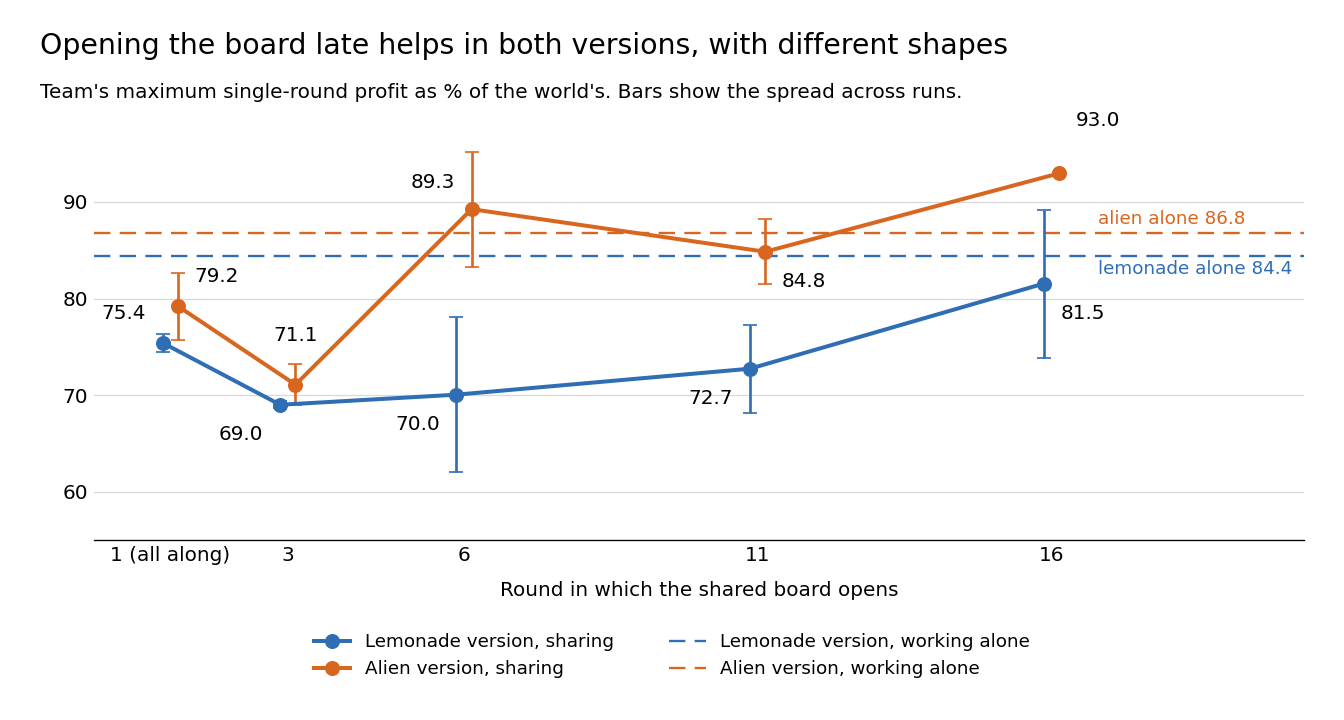
\includegraphics[width=0.78\linewidth]{figures/fig_sharing_timing_runs.png}
  \caption{Team max as a share of the world's optimum, by the round in which the shared board opens.}
  \label{fig:timing}
  \figurenote{Blue is the lemonade framing and orange the alien framing. The dashed line in each colour is the working-alone level for that framing. GPT-5.6, eight worlds, two or three runs per world; bars show the standard deviation across runs.}
\end{figure}

\paragraph{Per-condition contrasts.}
Table~\ref{tab:percondition} gives each sharing condition's difference from working alone on every measure. On the max, no
sharing condition is above working alone in the lemonade framing. In the alien framing two are slightly above
it: sharing at rounds 6, 11 and 16 only, at \AliPeriodicMax\% against \AliSoloMax\% (difference
\AliPeriodicDiff{} points [\AliPeriodicLo, \AliPeriodicHi], $p=\AliPeriodicP$), and the stay-different
instruction, at \AliProtocolMax\% (\AliProtocolDiff{} points, $p=\AliProtocolP$). Neither is distinguishable
from working alone. The first gap comes down to one extra world-run in which the team reached the best
location, \AliPeriodicReached{} against \AliSoloReached{} for working alone; the condition was ahead of
working alone in two of its three runs and behind in the third, and in the lemonade framing the same condition
is \LemPeriodicMax\% against \LemSoloMax\%, below working alone. We therefore read both as level with working
alone, not better. What the two have in common is that they are the two sharing designs that keep exploration
near the working-alone level.

\paragraph{Replication on sixteen further worlds.}
Because the test over eight worlds cannot separate a gap of a few points from zero, we ran the periodic-board
condition and working alone on sixteen further worlds that no condition had touched, three runs per world, in
both framings, with the analysis fixed before each run. Table~\ref{tab:worlds24} gives the paired differences
on the new worlds, on the pilot worlds and on all 24. The pre-specified primary result, in both framings, is
that the periodic board is level with working alone on the max. In the lemonade framing it is \WLAllMax{}
points relative to working alone over all 24 worlds [\WLAllMaxLo, \WLAllMaxHi], $p\WLAllMaxP$, with
\WLAllMaxUp{} worlds up and \WLAllMaxDown{} down; the \WLPilotMax{}-point deficit on the pilot worlds did not
reproduce on the new ones (\WLNewMax{} points). In the alien framing it is \WAllMax{} points [\WAllMaxLo,
\WAllMaxHi], $p\WAllMaxP$, and the small advantage seen on the pilot worlds did not reproduce either
(\WNewMax{} points on the new worlds); both arms reached the best location in the same share of world-runs,
\WAllReachedArm\% against \WAllReachedSolo\%. The other two effects reproduced in both framings and are now
reliable on 24 worlds: cumulative earnings \WLAllSum{} points [\WLAllSumLo, \WLAllSumHi] in the lemonade
framing and \WAllSum{} [\WAllSumLo, \WAllSumHi] in the alien framing, both $p\WAllSumP$; distinct setups
\WLAllUniq{} [\WLAllUniqLo, \WLAllUniqHi] and \WAllUniq{} [\WAllUniqLo, \WAllUniqHi], both $p\WAllUniqP$, with
the count lower in \WLAllUniqDown{} and \WAllUniqDown{} of the \WAllUniqN{} worlds.

\begin{table}[t]
  \centering
  \caption{Sharing at rounds 6, 11 and 16 relative to working alone, paired over worlds, both framings. Three runs per world. Max and cumulative earnings in percentage points of the optimum; distinct setups in counts; reached best location in percentage points of world-runs.}
  \label{tab:worlds24}
  \scriptsize
  \setlength{\tabcolsep}{3.5pt}
  \begin{tabular}{l l rc rc rc}
\toprule
 & & \multicolumn{2}{c}{16 new worlds} & \multicolumn{2}{c}{8 pilot worlds} & \multicolumn{2}{c}{All 24 worlds} \\
\cmidrule(lr){3-4} \cmidrule(lr){5-6} \cmidrule(lr){7-8}
Framing & Measure & Difference [95\% CI] & $p$ & Difference [95\% CI] & $p$ & Difference [95\% CI] & $p$ \\
\midrule
Lemonade & Max & +0.8 [-6.9, +8.5] & 0.828 & -5.6 [-21.7, +10.5] & 0.438 & -1.3 [-8.1, +5.4] & 0.684 \\
 & Cumulative & +10.4 [+6.3, +14.5] & $<$0.001 & +7.2 [+0.5, +13.9] & 0.023 & +9.3 [+6.0, +12.6] & $<$0.001 \\
 & Distinct setups & -6.9 [-9.7, -4.1] & $<$0.001 & -5.8 [-9.2, -2.3] & 0.031 & -6.5 [-8.5, -4.5] & $<$0.001 \\
 & Reached best location (\%) & -0.0 [-15.9, +15.9] & 1.000 & -12.5 [-42.1, +17.1] & 0.531 & -4.2 [-17.5, +9.2] & 0.668 \\
\addlinespace
Alien & Max & -0.6 [-4.8, +3.5] & 0.875 & +2.9 [-12.7, +18.5] & 0.703 & +0.6 [-4.6, +5.7] & 0.838 \\
 & Cumulative & +5.9 [+2.5, +9.4] & 0.002 & +11.5 [+4.9, +18.1] & 0.016 & +7.8 [+4.7, +10.9] & $<$0.001 \\
 & Distinct setups & -7.5 [-9.2, -5.8] & $<$0.001 & -5.2 [-8.6, -1.9] & 0.023 & -6.7 [-8.2, -5.2] & $<$0.001 \\
 & Reached best location (\%) & -2.1 [-12.3, +8.1] & 1.000 & +4.2 [-23.5, +31.8] & 1.000 & -0.0 [-10.2, +10.2] & 1.000 \\
\bottomrule
\end{tabular}
  \figurenote{The sixteen new worlds are not the pilot worlds' equals in level: in the alien framing they are easier for both arms (working alone reaches a max of \WNewMaxSolo\% against \AliSoloMax\%) and in the lemonade framing harder (\WLNewMaxSolo\% against \LemSoloMax\%), so levels are not comparable across the two sets; the paired differences are. The same sixteen worlds are used in both framings.}
\end{table}

\begin{table}[t]
  \centering
  \caption{Each sharing condition's difference from working alone, paired within worlds, all runs. Max and cumulative earnings in percentage points; distinct setups in counts. $^{\ast}$ marks $p<0.05$ on the exact sign-flip test.}
  \label{tab:percondition}
  \small
  \setlength{\tabcolsep}{4pt}
  \begin{tabular}{l ccc ccc}
\toprule
 & \multicolumn{3}{c}{Lemonade framing} & \multicolumn{3}{c}{Alien framing} \\
\cmidrule(lr){2-4} \cmidrule(lr){5-7}
Difference from working alone & Max & Cumulative & Distinct & Max & Cumulative & Distinct \\
\midrule
Sharing all along & -9.0 & +11.2$^{\ast}$ & -20.1$^{\ast}$ & -15.6 & +10.4 & -23.0$^{\ast}$ \\
Sharing after 2 private rounds & -15.4 & +5.1 & -20.9$^{\ast}$ & -10.0 & +12.2 & -22.0$^{\ast}$ \\
Sharing after 5 private rounds & -14.4 & +5.2 & -16.4$^{\ast}$ & -12.0 & +8.3 & -19.4$^{\ast}$ \\
Sharing after 10 private rounds & -11.7 & +5.1 & -10.9$^{\ast}$ & -3.2 & +8.8$^{\ast}$ & -11.4$^{\ast}$ \\
Sharing after 15 private rounds & -2.9 & +3.4 & -3.3 & -2.3 & +4.6 & -5.1$^{\ast}$ \\
Sharing at rounds 6, 11 and 16 only & -5.6 & +7.2$^{\ast}$ & -5.7$^{\ast}$ & +2.9 & +11.5$^{\ast}$ & -5.2$^{\ast}$ \\
Sharing, told to stay different & -5.9 & +13.6 & -1.4 & +1.5 & +18.9$^{\ast}$ & -2.6 \\
One agent at a time & -3.2 & +18.4$^{\ast}$ & -24.4$^{\ast}$ & -14.4 & +13.4 & -26.9$^{\ast}$ \\
\bottomrule
\end{tabular}
\end{table}

\paragraph{Replication on a second model.}
To check that the pattern is not specific to GPT-5.6, we ran working alone, sharing all along and sharing at
rounds 6, 11 and 16 on Claude Opus 5.5, in both framings, on the eight pilot worlds, two runs per world, with
the analysis fixed before the runs. Table~\ref{tab:claude} puts the paired
differences beside GPT-5.6's on the same worlds. The drop in exploration reproduces in every cell: sharing all
along cuts distinct setups by \CLemUniqShare{} in the lemonade framing and \CAliUniqShare{} in the alien
framing, both $p\CLemUniqShareP$, and the periodic board by less. Cumulative earnings are higher under sharing
in all four cells, reliably so for sharing all along in the alien framing (\CAliSumShare{} points,
$p\CAliSumShareP$). On the max the two models differ in one place. For Claude, sharing all along lowers the max
in the lemonade framing by \CLemMaxShare{} points [\CLemMaxShareLo, \CLemMaxShareHi], a larger drop than
GPT-5.6's, with the team reaching the best location in \CLemReachedShareArm\% of world-runs against
\CLemReachedShareSolo\% working alone; in the alien framing it is level with working alone (\CAliMaxShare{}
points), where GPT-5.6 showed a drop. The periodic board is level with working alone on the max in both
framings for Claude (\CLemMaxPeriodic{} and \CAliMaxPeriodic{} points), as it is for GPT-5.6 on 24 worlds.
Claude working alone also reaches a higher max than GPT-5.6 in the lemonade framing (\CLemMaxShareSolo\%
against \LemSoloMax\%), so the two models search differently; what they share is that visibility reduces
search, raises earnings, and never raises the ceiling.

\begin{table}[t]
  \centering
  \caption{Second model. Each sharing condition's difference from working alone, paired over the eight pilot worlds, for Claude Opus 5.5 (two runs per world) and GPT-5.6 (two or three runs per world) on the same worlds. Max and cumulative earnings in percentage points of the optimum; distinct setups in counts. $^{\ast}$ marks $p<0.05$ on the exact sign-flip test.}
  \label{tab:claude}
  \scriptsize
  \setlength{\tabcolsep}{3pt}
  \begin{tabular}{l l cc cc}
\toprule
 & & \multicolumn{2}{c}{Claude Opus 5.5} & \multicolumn{2}{c}{GPT-5.6} \\
\cmidrule(lr){3-4} \cmidrule(lr){5-6}
Framing & Measure & Sharing all along & Sharing at 6, 11, 16 & Sharing all along & Sharing at 6, 11, 16 \\
\midrule
Lemonade & Max & -14.9 [-29.3, -0.6] & -3.1 [-11.0, +4.9] & -9.0 [-25.3, +7.2] & -5.6 [-21.7, +10.5] \\
 & Cumulative & +4.0 [-8.2, +16.3] & +7.0 [-1.8, +15.7] & +11.2$^{\ast}$ [+3.1, +19.4] & +7.2$^{\ast}$ [+0.5, +13.9] \\
 & Distinct setups & -18.8$^{\ast}$ [-21.5, -16.1] & -6.1$^{\ast}$ [-8.1, -4.0] & -20.1$^{\ast}$ [-26.9, -13.3] & -5.7$^{\ast}$ [-9.2, -2.3] \\
\addlinespace
Alien & Max & +3.0 [-10.1, +16.0] & -5.1 [-13.5, +3.2] & -7.6 [-30.9, +15.7] & -3.1 [-16.5, +10.2] \\
 & Cumulative & +7.5 [-2.0, +16.9] & +3.5 [-1.9, +8.9] & +17.2$^{\ast}$ [+3.5, +30.9] & +8.5$^{\ast}$ [+3.7, +13.3] \\
 & Distinct setups & -9.2$^{\ast}$ [-15.5, -2.9] & -1.6 [-5.4, +2.3] & -21.8$^{\ast}$ [-24.7, -18.9] & -5.6$^{\ast}$ [-9.6, -1.5] \\
\bottomrule
\end{tabular}
\end{table}

\paragraph{A longer horizon.}
Whether the trade between earning and finding is a property of the game or of stopping at round 20 can be
tested directly. We ran working alone and sharing all along for 60 rounds, in both
framings, on the eight pilot worlds, three runs per world, with the analysis and a decision rule fixed before
the runs. These are new games, not continuations: every prompt says ``Round $r$ of 60'', and an agent that
believed round 20 was the last played its last rounds accordingly. Table~\ref{tab:h60} gives the paired
differences over the whole 60-round game, over rounds 21 to 60 alone, and, for comparison, in the 20-round
game on the same worlds. The two framings move in opposite directions. With the letter, time favours sharing.
The drop in the max closes from \HLemMaxGame{} points in the 20-round game to \HLemMaxFull{} points
[\HLemMaxFullLo, \HLemMaxFullHi] over 60 rounds, as sharing teams eventually leave the recommended location
and reach the best one in \HLemReachedFullArm\% of world-runs against \HLemReachedFullSolo\% working alone,
while the cumulative lead of sharing grows to \HLemSumFull{} points [\HLemSumFullLo, \HLemSumFullHi]
($p\HLemSumFullP$, \HLemSumFullUp{} of 8 worlds) and is still \HLemSumLate{} points in rounds 21 to 60.
Without the letter, time favours the lone agents. The drop in the max does not close (\HAliMaxFull{} points
[\HAliMaxFullLo, \HAliMaxFullHi]; \HAliReachedFullArm\% of sharing world-runs reach the best location against
\HAliReachedFullSolo\% working alone), and the cumulative lead of sharing shrinks from \HAliSumGame{} points
in the 20-round game to \HAliSumFull{} points over 60 rounds [\HAliSumFullLo, \HAliSumFullHi], and is
\HAliSumLate{} points in rounds 21 to 60, with \HAliSumLateDown{} of 8 worlds favouring working alone. The
collapse of exploration is unchanged by the horizon: sharing cuts distinct setups by \HLemUniqFull{} and
\HAliUniqFull{} over 60 rounds, and in rounds 21 to 60 a sharing team tries \HLemUniqLateArm{} and
\HAliUniqLateArm{} distinct setups against \HLemUniqLateSolo{} and \HAliUniqLateSolo{} for three agents working
alone. Being told the game is longer also changes early play. In the first 20 rounds of the 60-round game,
sharing teams in the lemonade framing reach a max of \ELemShareMaxHsixty\% against \ELemShareMaxHtwenty\% in
the 20-round game (\ELemShareMax{} points, $p\ELemShareMaxP$), and lone agents in both framings try more
distinct setups early (\ELemSoloUniq{} and \EAliSoloUniq{}, $p\ELemSoloUniqP$ and $p\EAliSoloUniqP$).

\begin{table}[t]
  \centering
  \caption{A longer horizon. Sharing all along relative to working alone, paired over the eight pilot worlds, GPT-5.6, three runs per world, in 60-round games and, for comparison, in the 20-round game on the same worlds. Max and cumulative earnings in percentage points of the optimum; distinct setups in counts; reached best location in percentage points of world-runs. $^{\ast}$ marks $p<0.05$ on the exact sign-flip test.}
  \label{tab:h60}
  \scriptsize
  \setlength{\tabcolsep}{4pt}
  \begin{tabular}{l l c cc}
\toprule
 & & 20-round game & \multicolumn{2}{c}{60-round game} \\
\cmidrule(lr){3-3} \cmidrule(lr){4-5}
Framing & Measure & rounds 1--20 & rounds 1--60 & rounds 21--60 \\
\midrule
Lemonade & Max & -9.0 [-25.3, +7.2] & -1.4 [-9.8, +7.0] & -1.4 [-9.8, +7.0] \\
 & Cumulative & +11.2$^{\ast}$ [+3.1, +19.4] & +18.2$^{\ast}$ [+11.6, +24.8] & +14.8$^{\ast}$ [+6.8, +22.8] \\
 & Distinct setups & -20.1$^{\ast}$ [-26.9, -13.3] & -40.5$^{\ast}$ [-46.2, -34.8] & -14.5$^{\ast}$ [-21.7, -7.2] \\
 & Reached best location & -20.8 [-53.9, +12.3] & -4.2 [-22.0, +13.7] & -4.2 [-22.0, +13.7] \\
\addlinespace
Alien & Max & -15.6 [-35.9, +4.7] & -19.0 [-41.0, +2.9] & -19.0 [-41.0, +2.9] \\
 & Cumulative & +10.4 [-1.9, +22.7] & +2.2 [-15.7, +20.1] & -3.0 [-23.5, +17.5] \\
 & Distinct setups & -23.0$^{\ast}$ [-25.9, -20.0] & -33.5$^{\ast}$ [-41.4, -25.7] & -11.7$^{\ast}$ [-17.5, -5.9] \\
 & Reached best location & -29.2 [-63.9, +5.6] & -33.3 [-72.8, +6.1] & -33.3 [-72.8, +6.1] \\
\bottomrule
\end{tabular}
\end{table}

\paragraph{Reproducibility.}
Figure~\ref{fig:intervals} and Table~\ref{tab:contrasts} compare the first run with the repeats. The three
headline contrasts have the same sign in the first run, in the repeats and in all runs, in both framings. Per
condition, the repeats fall on the same side of working alone as the first run in \AgreeSame{} of \AgreeOf{}
condition-measure-framing cells, and the four exceptions are cells within 7 points or 3 setups of zero both
times (Appendix~\ref{app:agree}). The repeats did not change any conclusion of the first run. They narrowed the
intervals on cumulative earnings and distinct setups enough to make both reliable in each framing on its
own, and they left the max where it was: a consistent drop that eight worlds cannot separate from zero.

\begin{figure}[t]
  \centering
  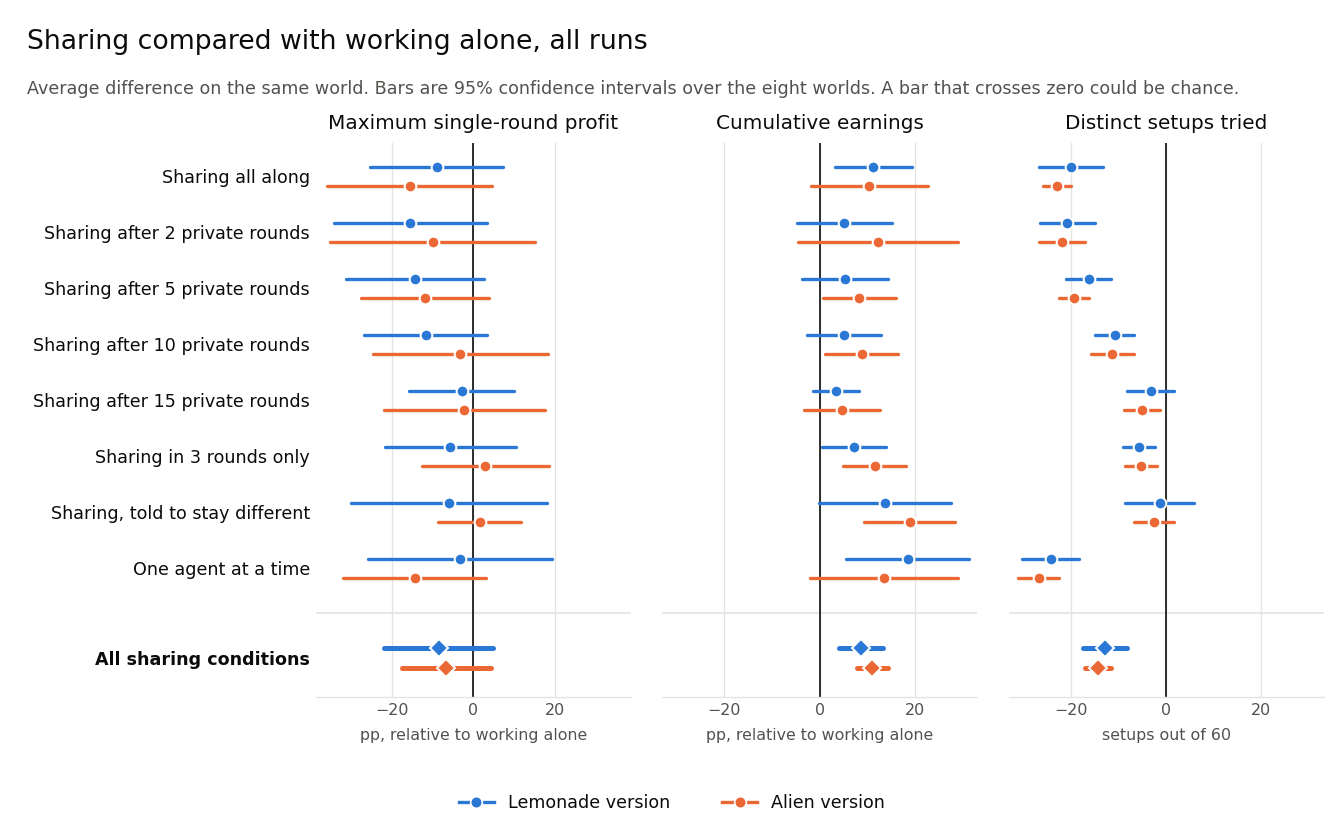
\includegraphics[width=0.95\linewidth]{figures/fig_sharing_intervals.png}
  \caption{Each sharing condition, and the mean of all sharing conditions, relative to working alone, with 95\% intervals, all runs.}
  \label{fig:intervals}
  \figurenote{Paired over the eight worlds; blue is the lemonade framing and orange the alien framing. For the pooled contrast in the bottom row, the intervals for cumulative earnings and distinct setups exclude zero in both framings and the interval for the max includes zero in both.}
\end{figure}
